\documentclass[11pt,a4paper,oneside]{book}

% Include the configuration file for layout.
\usepackage{setspace}
\usepackage{geometry}
\usepackage[toc]{appendix}
\usepackage{lipsum}
\usepackage[export]{adjustbox}
\usepackage[T1]{fontenc}
\usepackage{textcomp}
\usepackage{epsfig,graphics}
\usepackage{graphicx}
\usepackage{titlesec}
\usepackage{hyperref}
\usepackage{pgfplots}
\usepackage{listings}
\usepackage{numprint}
\usepackage[numbers]{natbib}
% \usepackage{refcheck}
\usepackage{chngcntr}
\usepackage{tikz}
\usepackage{wrapfig}
\usepackage{caption} % this makes clickable references to figure to to its top instead of the caption on the bottom

\usetikzlibrary{shapes}
\hypersetup{
    breaklinks, hidelinks,
    bookmarksnumbered=true,
    bookmarksopen=true,
    bookmarksopenlevel=1
}
\lstset{basicstyle=\small, frame=L, xleftmargin=10pt}
% make figures and listings start from 1 instead of with chapter number
\counterwithout{figure}{chapter}
\npthousandsep{\,}

%%%%%%%%%%%%%%%%%%%%%%%%%%%%%%%%%%%%%%%%%%%%%%%%%%%%%%%%%%%%%%%%%%%%%%%%%%%%%%
% Details of your dissertation
%%%%%%%%%%%%%%%%%%%%%%%%%%%%%%%%%%%%%%%%%%%%%%%%%%%%%%%%%%%%%%%%%%%%%%%%%%%%%%

% Fill in the following fields.
\newcommand{\projectTitle}{A user friendly filesystem prototype with strong integrity guarantees}
\newcommand{\fullname}{Boyan Nikolaev Karatotev}
\newcommand{\degreeTitle}{BSc Computer Science}
% e.g. "BSc Computer Science"
\newcommand{\session}{2021/22}
% "Session" means the academic year, i.e. 2021/22.
\newcommand{\module}{COMP3931 Individual project}
% e.g. "COMP3931 Individual Project".

%%%%%%%%%%%%%%%%%%%%%%%%%%%%%%%%%%%%%%%%%%%%%%%%%%%%%%%%%%%%%%%%%%%%%%%%%%%%%%
% Change the geometry of the page to have a 25 mm binding edge
%%%%%%%%%%%%%%%%%%%%%%%%%%%%%%%%%%%%%%%%%%%%%%%%%%%%%%%%%%%%%%%%%%%%%%%%%%%%%%
\geometry{
    a4paper,
    total={210mm,297mm},
    left=25mm,
    right=25mm,
    top=25mm,
    bottom=20mm,
}

%%%%%%%%%%%%%%%%%
% own commands
%%%%%%%%%%%%%%%%%%
\newcommand{\monospace}{\texttt}
\newcommand{\syscall}[1]{\monospace{#1()}}
% TODO: make these work properly
\newcommand{\cauthor}[1]{\citeauthor{#1} \cite{#1}}
\newcommand{\cyear}[1]{\citeyear{#1} \cite{#1}}
\newcommand{\bplustree}{B\textsuperscript{+}-tree}

%%%%%%%%%%%%%%%%%%%%%%%%%%%%%%%%%%%%%%%%%%%%%%%%%%%%%%%%%%%%%%%%%%%%%%%%%%%%%%
% Commands to set the line spacing
%%%%%%%%%%%%%%%%%%%%%%%%%%%%%%%%%%%%%%%%%%%%%%%%%%%%%%%%%%%%%%%%%%%%%%%%%%%%%%
%\singlespacing
\onehalfspacing
%\doublespacing

%%%%%%%%%%%%%%%%%%%%%%%%%%%%%%%%%%%%%%%%%%%%%%%%%%%%%%%%%%%%%%%%%%%%%%%%%%%%%%
% Spacing for the chapter header
%%%%%%%%%%%%%%%%%%%%%%%%%%%%%%%%%%%%%%%%%%%%%%%%%%%%%%%%%%%%%%%%%%%%%%%%%%%%%%
\titleformat{\chapter}[display]
    {\normalfont\Huge\bfseries}{\vspace*{-1\baselineskip}\chaptertitlename\ \thechapter}{15pt}{\huge}
\titlespacing*{\chapter}{0pt}{0pt}{15pt}

\renewcommand\bibname{References}

%%%%%%%%%%%%%%%%%%%%%%%%%%%%%%%%%%%%%%%%%%%%%%%%%%%%%%%%%%%%%%%%%%%%%%%%%%%%%%
% Some shortcuts that maybe useful
%%%%%%%%%%%%%%%%%%%%%%%%%%%%%%%%%%%%%%%%%%%%%%%%%%%%%%%%%%%%%%%%%%%%%%%%%%%%%%
\DeclareTextCommandDefault{\textcopyright}{\textcircled{c}}

%%%%%%%%%%%%%%%%%%%%%%%%%%%%%%%%%%%%%%%%%%%%%%%%%%%%%%%%%%%%%%%%%%%%%%%%%%%%%%
% Bibliography style: choose one and make sure you have the relevant .bst file
%%%%%%%%%%%%%%%%%%%%%%%%%%%%%%%%%%%%%%%%%%%%%%%%%%%%%%%%%%%%%%%%%%%%%%%%%%%%%%
\bibliographystyle{plainnat}


%%%%%%%%%%%%%%%%%%%%%%%%%%%%%%%%%%%%%%%%%%%%%%%%%%%%%%%%%%%%%%%%%%%%%%%%%%%%%%
% Layout for the front cover !!!!! YOU SHOULD NOT HAVE TO CHANGE THIS!!!!!
%%%%%%%%%%%%%%%%%%%%%%%%%%%%%%%%%%%%%%%%%%%%%%%%%%%%%%%%%%%%%%%%%%%%%%%%%%%%%%

\newcommand{\frontcover}{
    % The title page:
    \begin{titlepage}
    \newgeometry{left=25mm,right=25mm,top=45mm,bottom=0.1cm}

    \begin{minipage}[t]{6cm}
    \noindent\textbf{\Large{School of Computing}}\\
    {\fontfamily{ptm}\selectfont
        \uppercase{faculty of engineering and physical sciences}
    }
    \end{minipage}
    \hfill
    \begin{minipage}[t]{7cm}
    \vspace*{-15pt}
    
\includegraphics[scale=0.2,right]{logo_black.png}
    \vspace*{-1pt}
    \end{minipage}

    \noindent\makebox[\linewidth]{\rule{\paperwidth}{0.4pt}}

    \centering
    \vspace*{20mm}
    \textbf{\huge Final Report}\\
    \vspace*{20mm}
    \textbf{\Large\projectTitle}\\
    \vspace*{10mm}
    \textbf{\large\fullname}\\
    \vspace*{10mm}
    \textbf{Submitted in accordance with the requirements for the degree of}\\
    \textbf{\degreeTitle}\\
    \vspace*{10mm}
    \session\\
    \vspace*{10mm}
    \module\\
    \restoregeometry
    \end{titlepage}
}

%%%%%%%%%%%%%%%%%%%%%%%%%%%%%%%%%%%%%%%%%%%%%%%%%%%%%%%%%%%%%%%%%%%%%%%%%%%%%%
% Define a new environment for the dissertation summary
%%%%%%%%%%%%%%%%%%%%%%%%%%%%%%%%%%%%%%%%%%%%%%%%%%%%%%%%%%%%%%%%%%%%%%%%%%%%%%
\newenvironment{metachapter}[1]
 	{\cleardoublepage \null
 		\begin{center}%
            \chapter*{#1}
			% \textbf{#1}
            \label{ch:#1}
            \addcontentsline{toc}{section}{\nameref{ch:#1}}
		\end{center}}%
	{\vfill \null }


\begin{document}

% The prelude is everything up to the start of chapter 1, and is contained
% in a file called "prelude.tex".
\pagenumbering{roman}
\frontcover

\clearpage

\noindent The candidate confirms that the following have been submitted.\\

% Below are examples of what your deliverables may be,
% but since every project is different, not all deliverables
% apply to all projects. Having said that, you should have
% the 'Final Report' deliverable, and most projects will also
% have a link to an online software repository.

\begin{table}[ht!]
\begin{tabular}{|p{0.3\textwidth}|p{0.3\textwidth}|p{0.3\textwidth}|}
\hline 
Items & Format & Recipient(s) and Date \\ 
\hline 
Final Report & PDF file & Uploaded to Minerva (DD/MM/YY) \\ 
\hline 
<Example> Scanned participant consent forms & PDF file / file archive & Uploaded to Minerva (DD/MM/YY) \\ 
\hline 
<Example> Link to online code repository & URL & Sent to supervisor and assessor (DD/MM/YY) \\ 
\hline 
<Example> User manuals & PDF file & Sent to client and supervisor (DD/MM/YY) \\ 
\hline 
\end{tabular} 
\end{table}


\vfill

\noindent The candidate confirms that the work submitted is their own and the appropriate credit has been given where reference has been made to the work of others.

\vfill

\noindent I understand that failure to attribute material which is obtained from another source may be considered as plagiarism.

\vfill

% Sign this with a pen for all of the hard copies before you hand
% them over to the SSO. If for any reason the submission of final reports
% is online-only, replace the '\rule{}{}' command with your name.
\flushright(Signature of Student) \rule{50mm}{1pt}
\flushleft

\vfill

\textcopyright~\session~The University of Leeds and~\fullname
% Summary

\begin{dissertationsummary}
Over the years UNIX like operating systems and their filesystems have gone a
long way. Numerous advances achieve very high degrees of resource utilisation
with robust and well thought out features. A major consideration throughout has
been drive unreliability. Any drive is prone to failure and even when function
may misbehave in an undetectable manner. To ensure data integrity there exist
many solutions, some better than others. Notably ext4 ensures filesystem
consistency even if data is unaccounted for while ZFS considers every
eventuality even if at the cost of substantial complexity. At the same time
simplistic solutions like arrays of disks (RAID) go a long way to provide
redundancy.

All of these solutions have problems though. Ext4 does not checksum data, RAID
has a write hole issue and ZFS is incredibly complex. This presents a challenge
for less technically savvy home users who will not be aware of the pros and
cons of each or may simple be unable to administer them.

To that effect, this project proposes a new filesystem that attempts to collect
the good things of each of these while mitigating the major issues and making
it easy to use. It integrates modern techniques for ensuring data integrity
without compromising on performance by design.  It targets the ever so
ubiquious solid state drives to optimise for what is most likely to be in the
target field of laptops, office desktops and home servers.

The proof of concept implementation achieves very good integrity. All data is
stored with full redundancy to protect against any pattern of drive
misbehaviour. Any silent data corruption can be detected with secure hashes of
all blocks and restored from the redundant copies. The result is cost and
administratively competitive with a wide variety of other solutions so it is a
valid choice.

Its performance is suboptimal due to not including extents and prototype
implementation. The penalty for the lack of extents was unexpected and further
analysis is performed to find out the cause.

Nevertheless, the basic desgn is robust enough for the filesystem to become a
usable module. It is implemented as a FUSE module to ensure portability for
widespread and easy use. The shortcomings can be addressed without major
reworks and further iteration can be performed for a full product.

\end{dissertationsummary}

\clearpage
\centering\textbf{Acknowledgements}
\flushleft
<The page should contain any acknowledgements to those who have assisted with your work.
Where you have worked as part of a team, you should, where appropriate, reference to any contribution made by other to the project.>

\vspace{1cm}

Note that it is not acceptable to solicit assistance on `proof reading' which is defined as the
``the systematic checking and identification of errors in spelling, punctuation, grammar and sentence construction, formatting and layout in the test'';
see \texttt{https://www.leeds.ac.uk/secretariat/documents/proof\_reading\_policy.pdf}



% The contents
\tableofcontents

% The list of figures and tables. Optional.
%\clearpage
%\listoffigures
%\listoftables

\pagenumbering{arabic}


% Include as many chapters as you have.
% The "chapter1.tex" etc. files should be in a directory called "chapters"
% You can cite chapters by using '\ref{chapter1}', where the label must
% match that given in the 'label' command, as on the next line.
\label{background}
% Sections and sub-sections can be declared using \section and \subsection.
% There is also a \subsubsection, but consider carefully if you really need
% so many layers of section structure.
\chapter{Introduction and Background Research}

    \section{Introduction}

    % <A brief introduction suitable for a non-specialist, {\em i.e.} without
    % using technical terms or jargon, as far as possible. This may be
    % similar/the same as that in the 'Outline and Plan' document. The
    % remainder of this chapter will normally cover everything to be assessed
    % under the `Background Research` criterion in the mark scheme.>

    % Here is an example of how to cite a reference using the numeric system
    % \cite{parikh1980adaptive}.


    % Must provide evidence of a literature review. Use sections
    % and subsections as they make sense for your project.

% TODO: this is a temporary name
\chapter{Lit review}
    \section{The UNIX filesystem}
        \label{UFS}

        For the past 50 years the UNIX style operating system has been one of
        the most prevalent operating system architectures out there. The
        original UNIX brought about a simple and elegant template which is
        still with us to this day. It brough forward many novel ideas: wide
        hardware compatibility, simple and powerful system calls, a powerfull
        shell and minimal design and most importantly a file system
        \cite{UNIX}. All these features are still with us, largely unmodified,
        to this day, although greatly expanded and improved upon.

        The most important part, the filesystem, had an implementation akin to
        its interface - simple and elegant. It introduced several important
        concepts:

        From a programming view, a file is a linear sequence of bytes and can
        be controlled with just 4 system calls: \syscall{open} \syscall{read},
        \syscall{write} and \syscall{close}. No structure is enforced on it
        from the operating system. A file can be \syscall{open}ed by name to
        get a handle to it. Programs can \syscall{read} all of its contents and
        \syscall{write} back anything new. The operating system maintains an
        offset showing the current location within the file, so sequential
        calls to \syscall{read} and \syscall{write} begin operation from that
        location and increment it by the amount they modified. No limit is
        imposed on file size, so writing past the end of the file increases it.
        A file must be \syscall{close}ed after use.

        From an implementation view, every file has an i-number. This is a
        number that uniquely identifies this file, regardless of its path or
        location. It is essentially the pointer to the file in the table of
        files, called an i-list (or i-table more recently).

        Each entry in the i-list is an i-node (modernly shortened to just
        inode). The inode is essentially the header for the file itself, it has
        all metadata including pointers to the actual data.

        To make this flat list of files into a usable tree, special files are
        introduced, called directories, marked by a special bit in the inode.
        The directory is a file whose contents have a special format: a list of
        2-tuples (name, i-number), which denote that file number
        \textit{i-number} can be found in this directory under name
        \textit{name}. Directories are special in that they cannod be read and
        written directly, rather special system calls must be used for the
        operating system to report its contents. The exact method is slightly
        involved and not relevant for this dissertation, but it is sufficent to
        say that there are simple library functions roughly equvalent to those
        for normal files.

        File names are alphanumeric strings of any length. To denote that a
        file is contained within a directory, a single forward slash ("/") is
        used, meaning whatever is on the right of it is contained on the
        directory named on the left. This can be repeated an unlimited number
        of times. The root directory has no name \textit{per se}, hence any
        path refering to it starts with a slash, for example
        \textit{/file/in/root}.

        File number 1 is defined to be the the root directory to bootrstrap the
        search and inode 0 does not exist.

        An important, but not user visible detail (in any way) is that the
        filesystem has a list of free blocks (called the free list), to denote
        which space is unused by the system, where a block is a fixed chunk of
        space on disk.


    \section{Evolution of implementation}

        \subsection{UFS}

            Initially, this model had a very simple implementation. The
            original UNIX used a linear, fixed size i-list. An inode had 13
            pointers to data blocks, 10 of which point directly to data blocks,
            while the next 3 have 1, 2 and 3 levels of indirection
            respectively. The free list was a simple linked list, where
            each block had pointers to free blocks and a pointer to the
            next block in the list \cite{UNIX_implementation},
            \cite{UNIX_thompson}.

            Over time, however, it turned out that this arrangement was very
            inefficient. In particular, data blocks for a file lacked locality,
            as did the i-numbers for files in the same directory. Additionally,
            the free list would become very scrambled in that sequential
            entries in the list may be wildly far apart on disk. All of these
            problems got exacerbated after prologned use. On top of all that,
            due to hard drives (the main storage medium) being a physical
            spinning platter with a head that has to move to the track on drive
            and wait for the block to come under it (operation knows as
            "seek"), seek times for arbitrary blocks was large. As a result,
            throughput could be as low as 4\% \cite{FFS}.


        \subsection{FFS}

            % maybe mention that increasing block size decreases the need for
            % indirection
            \citeauthor{FFS} proposed many improvements to improve performance.
            For a start, block size was increased 8 fold from 512 bytes to 4096
            (or even 8192), which improved locality and reduced seek times,
            essentially for free, although extra complexity was introduced to
            minimise wasted space from small files. Further, blocks were
            grouped together into cylinder groups, where a cylinder is a
            physical feature of a hard drive, blocks on which have very good
            sequential performance.  Then, policies were introduced to keep
            data blocks of a file and inodes in a directoy sequential and on
            the same cylinder group where possible. Finally, the free list
            became a bitmap of a fixed size, eliminating the scrambling of
            supposedly sequential entries that further degrade performance.

            The result was that \citeauthor{FFS} measured an increase in disk
            bandwidth utilisation of about an order of magnitude without an
            increase in wasted space.

            % TODO: do i need this
            % An important note is that cylinder groups include redundant copies
            % of various metadata to increase resiliance to data loss from damage
            % to the disk.

            % Another important note is that filesystems which are near their
            % capacity suffer greatly decreased performance.

        \subsection{LFS}

            With advances in software and hardware, by \citeyear{IO_bottleneck}
            file access and reliability patterns became apparent. Especially
            for office use, small reads and writes dominate the workload. The
            physical nature of spinning hard drives make such operations costly
            when performed in a random manner. To imporove performance, caching
            is identified as a substantial improvement, which has been wildly
            used since \cite{Linux_caching}, \cite{IO_bottleneck}.


            However, \citeauthor{IO_bottleneck} points out some issues with
            such an approach: a system crash or a power outage puts the
            contents of such a cache in jeopardy. This is not a problem for a
            read cache, but a write cache loss can be catastraphic. This brings
            reliability into the picture and balancing performance for
            reliability becomes a key factor.

            Further, \citeauthor{IO_bottleneck} argues that such caching shifts
            the IO pattern from mostly random reads to mostly writes in
            occasional big bursts of relatively large amount of data.
            Maintaining the usual layout of filesystems popular so far does not
            make use of this fact, so the author suggests structuring the
            filesystem as a log - an append-only structure which wraps around
            once it fills up. This gives locality to files that are used
            together, utilises the burst nature of writes and recovery is easy
            - only the end may be corrupted \cite{IO_bottleneck}.

            It must be noted that maintaining a fraction of the disk free is
            once again emphasised as critical for good performance.

            \citeauthor{LFS}, reiterates the necessity of asynchronous writes
            (and therefore a cache). In LFS \cite{LFS}, based on
            \cite{IO_bottleneck}, the inode structure is kept exactly the same
            as in FFS (including the data block arrangement), but its layout
            policy was redically different. First, the i-list is now a regular
            file, but only contains addresses to where the actual inode can be
            found. The inode itself and its data are laid our sequentially to
            improve performance and the free list is done away with. Instead,
            the disk is split into large chunks of free continuous space -
            \textbf{extents} (called segments in LFS) - which contain a single
            block of metadata that includes that information.  Special care is
            taken to maintain these chunks large.  This is done to reduce
            fragmentation and to allow a better likelyhood for sequential
            accesses. It is important to note, that the idea for extents
            remains present to this day.

            New data is written in a log fashion. There are several fixed
            places where a pointer to the i-list is stored and there is a
            single fixed place that is dedicated to storing the last known good
            head of the log. This ensures reliability.

        \subsection{WAFL}

            With time reliability becomes an ever growing concern, both from a
            techincal and from a human perspective. The idea of snapshots
            contributes to both of these.

            Snapshots are read-only copies of the entire file system. Many of
            them are kept, allowing for old versions of files to be viewed in
            case of deletion. WAFL uses copy-on-write for disk blocks to avoid
            duplicating data \cite{WAFL}. Snapshots are essentially pointers to
            these blocks, hence a new snapshot consumes space only after data
            is modified. Block are freeded after all references to them are
            freed too.

            Besides file versioning, snapshots are useful for backups on the
            live system, since they are pretty much free on WAFL.


            The way WAFL implemnts the copy-on-write is by creating a tree of
            blocks, where the root is a known fixed block. Then it has all
            metadata (like i-list and free list) be a file too. The inodes of
            all of these files are stored in an inode file, whole inode itself
            is stored in the root block. This way every single bit of info
            required for the filesystems operation is connected in a rooted
            tree and copying the root block makes a snapshot. Modifying any
            other block requires copying to a new location with the
            modificaiton only on the new copy and modifying the reference to
            it. Modifying the reference requires the same operation, which
            eventually bubbles up to the root block which can be modified in
            place.

            The benefit of this approach is that the filesystem is always
            consistent. At no point is any data modified in place, meaning a
            crash cannot cause corruption. Rather a new copy is built somewhere
            in free space and only "added" to the filesystem when the whole
            branch of the tree is complete. Writing a single block is assumed
            to be atomic \cite{???}, so updating the root an all or nothing
            operation, limiting the impact of a crash to only some data loss
            that hasn't had the time to be commited to disk.

    \section{EXT4}

        The most modern version of the ext filesystem, ext4, is native and
        usually default on Linux. It integrates a lot of the improvements over
        the years while maintaining the same general idea. Since it was
        developed for (and by) Linux, which is a UNIX derivative, the ext
        family follows closely the same principles present over 50 years ago in
        UFS (section \ref{UFS}).

        It is a good benchmark for modern filesystems as it is the default on
        many (if not most) major Linux ditributions
        \cite{https://wiki.debian.org/FileSystem},
        \cite{https://access.redhat.com/documentation/en-us/red_hat_enterprise_linux/6/html/performance_tuning_guide/s-storage-fs}.
        It is actively maintained
        \cite{https://www.spinics.net/lists/linux-ext4/} and very mature, first
        appearing in version 2.6.19 in 2006
        \cite{http://www.h-online.com/open/features/Kernel-Log-Higher-and-Further-The-innovations-of-Linux-2-6-28-746805.html}.
        Finally, unlike its most direct competitiors by the likes of Windows'
        NTFS and MacOS' APFS, it is free and open source, so code and
        documentation are readily available.
    \section{Data integrity}

        % TODO: validate from paper, becase most of this is my general
        % knowledge (espcially parity calculation)
        \subsection{RAID}

            Non-volatile storage mediums have historically been orders of
            magnitude slower than volatile memories like RAM which are
            themselves much slower than CPUs and their caches \cite{raid has a
            Frank87, Stevens81}. Disk arrays are an attempt to increase IO
            performance and bridge that gap. However, drives are inherently
            unreliable \cite{pls (backblaze is a killer source)}, so putting
            many of them together exacerbates the problem \cite{maybe also
            raid. he has an MTTF caluclation}.  RAID is one solution for the
            problem of drive reliability \cite{RAID}. As its name suggests,
            RIAD adds redundancy to disk arrays. Popular RAID arrangements are
            RAID 1 and RAID 4/5.

            RAID 1 is two drives acting as one, effectively a mirror. If one of
            them fails the other is a perfect copy.

            RAIDs 4 and 5 are very similar. Both calculate extra parity for
            each block (by XORing the respective blocks on all disks together)
            and store it on an extra disk. The major difference is how they lay
            out parity across the disks. The result is that the array can lose
            a disk any of the disks while keeping all of the data intact. It
            has a benefit over RAID 1 in that it is cheaper.

            Even though not part of the original paper, RAID 6 is also very
            common. It is essentially RAID 5 but with more copies of the parity
            data (equal to the number of parity disks).

        \subsection{drive reliability}

            Drives are unreliable \cite{RAID}, \cite{Backblaze (idk which one)}.
            Due to their mechanical nature they wear out and stop working. They
            do this at an unpredictable rate for individual drives, but at
            relatively constant rates over large arrays \cite{Backblaze_stats}.
            Tools for monitoring drive health, like SMART, have been developed
            to combat the issue and are in general a good indicator for the
            likelyhood of loss of the drive.

            However, drive failure is not binary. They do not work flawlessly
            until such a time as to not work at all \cite{2D_RAID}. Individual
            sectors develop errors over time, failing to be read or written to.
            Drives try to combat the issue by keeping an array of spare sectors
            that replace misbehvaing ones when detected. To determine if a
            sector is misbehvaing in the first place, drives employ ECC codes
            \cite{data_corruption_storage_stack, although maybe someone else}.

            However, despite all the best efforts of drives and their
            manufacturers, drives still cannot be relied upon to report correct
            data all of the time \cite{data_corruption_storage_stack}.
            Occasionally, they will report an unrecoverable error to the
            operating system. Even more rarely, drives will return incorrect
            data without indicating errors. As a consequence, individual drives
            are never relied upon for the data to be present and intact and
            other techniques are always employed to ensure both of these
            independently \cite{LTT_data_loss?}.

            SSDs and flash storage in general are a similar tale. As
            \citeauthor{2D_RAID} puts it: "Flash is basically garbage. It
            barely works. We tolerate it because its fast" \cite{2D_RAID}. They
            employ similar techniques as spinning hard drives and suffer
            similar problems as them \cite{flash_large_scale},
            \cite{flash_reliability}. Their failure patterns are substantially
            different but the end result is the same - unrecoverable errors
            that would lead to data loss if not accounted for outside the
            drive.

        \subsection{At scale}

            A unique case for data reliability are datacenters for which data
            loss is not an option. They also operate at massive scales, where
            conventional approaches break down or become severe bottlenecks.
            Hence many, if not most, of these companies have special bespoke
            arrangements to fulfil their needs.

            \subsubsection{Backblaze}

                Conveniently, Backblaze, a cloud storage provider, has an open
                approach to its infrastructure, frequently publishing in-depth
                information and open sourcing parts of their infrastructure.

                Their solution \cite{Backblaze_arch} to reliability is
                conceptually distributed RAID 6 over 20 drives, 3 of which are
                parity. However, they do not use conventional RAID. Instead,
                they use custom software to split files into chunks they call
                "shards" which are then stored on normal ext4 filesystems. The
                choice is motivated by the good reliability and performance of
                ext4 and that inverting the usual order of replication and
                filesystem allows them to protect against filesystem
                corruption.

                Additionally, every shard is checksummed to protect against
                data corruption. This is necessary because "once in a while
                they return the wrong data, or are just unable to read a given
                sector" \cite{Backblaze_arch} and software needs to be able to
                identify the error and recompute the data from the parity.

        \subsection{Caching}

            % TODO: you can't not cite this. LTT could be a source?
            % TODO: soft-updates seems to be part of caching system. Explain
            % modern caches and that they have been there since time immemorial

            Caching is an integral part of modern operating systems
            \cite{IO_bottleneck?}. All modern variants employ it in various
            very visible ways. Reads are routinely cached and so are writes
            although with extra care. This practice is so prevalent that
            opening files/programs the first time is frequently orders of
            magnitude slower than any subsequent access. In particular, it is
            essential in obtaining good, almost sequential, performance out of
            random small writes \cite{soft_updates}.

            Caching, however, is tricky especially on the write side. Besides
            the usual cache coherence issues, caching of writes for prologned
            periods of time can easily lead to data loss. To avoid this
            possibility while not diminishing the effectiveness of techniques
            like soft updates \cite{soft_updates}, operating systems have to
            perform a fine balancing act.

            Linux in particular caches aggresively \cite{its docs?}. Luckily,
            its VFS layer implements this in an abstract manner, so individual
            filesystems do not need to implement it themselves. Nevertheless,
            they frequently need to be aware of it and in rare cases, like ZFS
            (\ref{ZFS}), they need special behaviour to implement some features
            of the filesystem.


\chapter{Design}

    \section{Methodology}
        \label{sec_methodology}

        % TODO: (some) duplicate with discussion
        Designing a filesystem is difficult and implemneting it even more so.
        For example, EXT4's documentation \cite{ext4_docs} is roughly 20000
        words of mostly major design features, and around 60000 lines of Linux
        kernel code. For this reason designing and implemneting this filesystem
        followed a peculiar process to reduce the risk of having an incomplete
        prototype by the submission deadline due to comlextiy.

        The process boils down a single principle: always have a working
        prototype. The idea is to start with the smallest and simplest
        implementation that works and then add individual features
        incrementally in a manner that always ends up with a working prototype.
        The plan was to initially complete the large amount of work to have
        \textit{any} filesystem and add geatures until time allowed. This way,
        no matter the unexpected obstacles in writing a filesystem and
        underestimation of effort turn out to be, there is always a submittable
        project to get some (even if lower) marks.

        % TODO: you can note that the kernel uses a similar thing with their patch
        % process. Think how I developed the arm internship code

    % TODO: is this necessary
    \section{Design goals}

        The backdrop for the design that follows are two goals: demonstrating
        integrity guarantees in a complete filesystem and maintaining
        simplicity of the design. The main reason behind them is the limited
        time and large potential scope of the project. It is intended that this
        project only be a prototype and not production ready infrastructure.
        This means avoiding special purpose data structures and sticking to the
        most basic solution that gives satisfactory results.

    \section{Metadata as files}
        \label{sec_files}

        The first design choice was that all metadata in the filesystem would
        be kept as a regular file instead of having special data structures for
        each, heavily inspired by WAFL (\ref{sec_WAFL}), although EXT4
        (\ref{sec_EXT4} also stores a substantial amount of metadata (but not
        all) as regular files too. This way they can all benefit from the
        underlying indexing method and substantially reduce implementation
        complexity. Further, this automatically solves the problem of how to
        allocate space for them.  For example, since the inode table is a file,
        there is no need make any special consideration for its initial size.
        It can grow as necessary, get spread throughput the filesystem as
        available and this approach will accommodate both edge cases equally
        well. On one end, where the filesystem has to store very few very large
        files, no space will be wasted towards an unused i-list. On the other
        end, where it has to store a very large amount of minuscule files, the
        ilist can grow to a substantial fraction of all storage, without
        running into an arbitrary limit.

    \section{Block size}
        \label{sec_block_size}

        % TODO: cite the all claim?
        As \citeauthor{FFS} explains (see \ref{sec_FFS}), larger block sizes
        improve throughput and reduce overhead, even on SSDs (see
        \ref{sec_hardware}). As a sensible default blocks are set to 4KiB in
        size, as viertually all filesystems do. It offers a good tradeoff
        between maximising IO performance and minimising overhead for things
        like free lists while still being small enough to not waste space if
        unused in small files.

        Extents (\ref{sec_LFS}) are a popular feature to increase throughput.
        This filesystem does not include them as they significantly increase
        complexity and their benefits only become apparent when combined with
        other features such as tree based free space tracking (described in
        \ref{sec_free_list}), more involved allocation algorithms like those in
        EXT4 (\ref{sec_EXT4}) or those that \citeauthor{ext4_space_maps}
        describes.

    \section{The free list}
        \label{sec_free_list}

        A popular way keep track of available free space is block bitmaps.
        Historically, many filesystems have frequently used it like FFS
        \cite{FFS}, WAFL \cite{WAFL} and more recently, EXT4
        \cite{ext4_space_maps} and HFS+ \cite{HFSplus}.  They are very space
        efficient, using only 256 KB per GB with 4KB blocks or about 0.02\%.
        Their small size allows them to be easily cached and kept up to date. A
        major drawback is that traversing these bitmaps is not particularly
        efficient as it usually devolves to some form of linear search,
        although some techniques can help mitigate this (for example storing
        extra bits of information about the closest free block).

        There are other techniques available, such as tracking free extents in
        a \bplustree like XFS \cite{XFS_scalability} or a proposed space map
        for EXT4 which relies on RB-trees \cite{ext4_space_maps}. Both of these
        approaches rely on space being managed in extents (see
        \ref{sec_block_size}).  Their major drawback of these approaches is
        their significantly increased complexity.

        In the end the classic bitmaps were selected. They work well enough,
        their implemntation is simple and a variety of allocation policies are
        possible with them. Alternative approaches depend on extents which are
        not supported and would introduce far too much extra complexity to the
        project for a limited benefit considering the generally basic design
        and time constraint. Time is well spend developing other features.

        Note that the free list isn't in the ilist, because of the bootstrap.

    \section{Superblock?}

        Say convention it's on block 1. It stores inode block nums to free list/ilist
        It's minimal and stores very little

        approaches rely on space being managed in extents. Their major drawback is
        the significantly increased complexity.

        In the end a file of the classic bitmap approach was selected. They
        work well enough, their implementation is simple and a variety of
        allocation policies are possible with them. Alternative approaches
        would introduce far too much extra complexity to the project for a
        limited benefit considering the generally basic design. Due to the time
        constraint, time is better spend developing other features.

    \section{The inode table and directories}

        Both structures are files containing a linear array of items. At the
        start of each file there is a small header which stores how many
        entries each file has. The only difference is in the items they store.
        The inode table contains inodes while directories store the usual
        (name, i-number) tuples. In both cases this is functionally equivalent
        to UFS (\ref{sec_UFS}).

        very different use cases.
        different arguments
        for simplicity keep linear
        made sense to unify

        Both structures serve very different purposes from a user facing
        perspective. However, the workload they need to complete is very
        similar. Both store a list of unordered entries. The directoy has to be
        searched to find the i-numbers of names. The inode table has to be
        searched to find a free entry to place a new inode. The only functional
        difference is that the inode table can be indexed to produce a result
        in constant time (and to that effect can be considered ordered, however
        the contents themselves have no particular order except their indices).

        As this filesystem strives for simplicity (\ref{sec_methodology}) it
        makes sense to unify the two structures. There exist bespoke
        implementations for both like ext4's Htrees for directories
        (\ref{sec_htree}). However, adding them introduces a lot of extra
        complexity which is undesiriable. Such features will not benefit the
        basic case much as the overwhelming majority of lookup in the inode
        table are i-number to inode resulutions (which are constant time as the
        index is reused in the table). Meanwhile, for home use, which this
        filesystem targets (\ref{sec_problem}), directories tend to not have a
        large number of files in them \cite{contents_strudy}. Therefore an
        imporovement in their speed will not be particularly noticable.

        As a result, a simple linear approach is adopted. It has pretty much
        the same benefits and the same drawbacks as those for the free list as
        the underlying structure is the same.

    \section{inode}

        Once again, to maintain simplicity, the inode contains only essentail
        information. This includes metadata like the owner's user and group
        IDs, the access permissions and creation/modifiaction timestamps.
        Non-metadata fields are the file's size and the head to the tree of
        data nodes, stored as a B-tree (see \ref{sec_design_btree}).

        The metadata is required to make a file understandable to Linux. It is
        also very simple to store as it has a known size and layout, is only
        stored in one place, and never referenced elsewehre. It could be
        reported as a fixed value (for example root as owner with full
        permissions for everything and the UNIX epoch as a creation timestamp)
        but omitting this information makes the filesystem unpleasant to debug,
        as it can be hard to tell if files with the exact same metadata are
        actually different or there is a bug.

        % TODO: should I include an strace trace of cat?
        The size and data fields are critical to implementing an inode and
        cannot be done away with. The data is obvious, since the file itself
        must be stored somewhere and the inode is the only place that
        references this. The need for the size is less apparent, since all
        systemcalls for manipulating a file, like \syscall{open},
        \syscall{read}, \syscall{write}, \syscall{lseek} and \syscall{close},
        do not reference it in any way. The data tree contains enough
        information for this value to not be stored explicitly.  For example,
        the tree will not contain a block for reading past the end of the file
        which will result in an error. However, basic programs like
        \monospace{cat} (which are one of the simplest way to access files
        \cite{TLDP_proc_access}) read the size of the file before making a
        request for its size (with \syscall{stat}) before reading it. This
        presents a challenge as, although it is possible to find out the size
        on each such call, it requires a nontrivial amount of code to do so.
        Needless to say, it is also unnecessarily inefficient. For the purpose
        of less code and a speed increase, it was deemed that storing this
        information and taking the slight complexity with it is worth it
        overall.

    \section{B-tree}
        \label{sec_design_btree}

        % TODO: chapter for FAT32 in backgroun? and double check exactly how it
        % did things to see if I said things right or if i'm subtly wrong
        Despite its ubiquity, the B-tree is not the only choice for storing
        data blocks for an inode. Simpler techniques have historically been
        used. Originally, UFS and FFS used a generic tree of staggered
        indirection (\ref{sec_UFS} and \ref{sec_FFS}). Another was FAT32 which
        used a linked list to describe all data blocks \cite{fat32}.

        The FAT32 scheme was experimented with, as it is quite a lot simpler
        than a full B-tree implementation. However, it proved very difficult to
        reason with on random accesses and performance was also abysmall
        (something FAT32 has always struggled with). Because of this it was
        decided to use a \bplustree from an external implementation. The B-tree
        is much more suited for this task (\ref{sec_btree}) and supports
        standard operations like insert, delete and lookup natively and
        performanlty.

    \section{Hardware considerations}
        \label{sec_hardware}

        % TODO: can reference ext4 data locality chapter to save on words
        A major focus for this filesystem was SSD instead of spinning
        mechanical hard drives. As a result, there are no major provisions for
        locality. This is because SSD random IO performance is almost in line
        with their sequential capabilities \cite{servethehome_review}. As a
        result, things are laid out in an arbitrary best fit fashion along the
        disk instead of considering future growth or access patterns.

        There is a single provision for increasing data locality. It is to have
        a minimum allocation size. This is because greater data locality "can
        increase the size of each transfer request while reducing the total
        number of requests" \cite{ext4_docs}. That minimum is set to 20
        blocks for a balance between high preallocation but not wasting much
        space.

    \section{Redundancy}

        The aim for the redundancy is "RAID with checksums", since RAID alone
        cannot be relied upon for data integrity (\ref{sec_RAID_problems}).

        First, to combat silent drive unreliability (see \ref{sec_reliability})
        all data must be checksummed. There are two choices for where this can
        happen: at the data structure level or at the block level. If done at
        the data structure level (i.e. every "pointer" would also include a
        checksum of its data), like EXT4 (\ref{sec_EXT4}, then there is a
        benefit that the data and its checksum are spatially separate (a
        provision ZFS has \ref{sec_ZFS}). However, this approach adds
        significant complexity for checks at all places. If done at the block
        level, then the rest of the filesystem can be ignorant about the
        existance of checksums and carry on as normal, reducing complexity and
        size requirements. Since this filesystem does not implement a tree of
        blocks, like ZFS (\ref{sec_ZFS}) does, this has the drawback that
        checksums are local to the data they protect. However, implemneting
        this is very trivial as it only needs to extend the block level
        interface and the entirity of the rest of the design can remain the
        same. This second approach is chosen for primarily this reason.

        For the question of where to store the checksum, there is only one
        solution that is not particularly involved. Storing the checksum within
        the block makes a corruption of the block extremely likely to corrupt
        the checksum too making it a very bad idea. The next best thing is
        having separate aggregate blocks that contain the checksums for as many
        blocks as possible just after them.

        Next comes the question of how much space to allocate for checksums.
        This is a space versus integrity tradeoff. On one hand the bigger the
        checksum the better since it allows for a lesser chance for collisions
        to mess things up. On the other hand, we want overhead to be as small
        as possible so that drives can be better utilised. For example, ext4
        allocates 4 bytes for each structure \cite{ext4_docs} but that is
        mostly for backwards compatibility and there simply not being room for
        more. ZFS stores 32 \cite{ZFS_docs}[basic\_cocepts/chechsums] for each
        block (usually 128KiB), which is estimated to be around 0.5\%
        \cite{ZFS_overhead}.

        For the scheme above of collating checksums for blocks in a separate
        block, a 4 byte checksum requires about 0.1\%, 16 bytes are 0.39\% and
        32 bytes are 0.78\%. A 0.1\% overhead would be idea, however this
        limits the choice of checksum algorithm severely (mostly Cyclic
        Redundancy Checks (CRCs) and Fletcher checksums
        \cite{embedded_checksums}). 64 bytes and more would be better for
        integrity but the overhead reaches single digit percent overhead which
        becomes significant. 32 bytes is the largest amount that is not
        significant enough to raise eyebrows. To make block numbers easy to
        compute this will mean every 128th block contains the checksums for the
        previous 127. The 128th place will be technically unused, so a checksum
        of the block itself for a bit of added integrity.

        Now, since checksums and data will be local to each other, the checksum
        algorithm must be as resiliant as possible to minimise the chance that
        a data corruption results in a checksum collision and the data is
        reported as unaltered. Even though the block checksums itself and that
        checksum is stored on the same block next to all the others, a corrupt
        block could feasibly alter an arbitrary checksum and the metachecksum
        at the same time. Since we are targetting SSDs (\ref{sec_SSD}) we may
        align checksum characteristics with SSD failure patterns.

        One way to measure SSD failures is with the raw bit error rate (RBER).
        The RBER is defined as the number of currupted bits per the number of
        total bits read \cite{flash_reliability}.
        \citeauthor{flash_reliability} take measurements over a vast number of
        drives with single-level cell (SLC, 1 bit per memory cell) and
        multi-level cells (MLC, 2 bits). They measure RBERs between $10^{-8}$
        and $10^{-5}$. \citeauthor{bit_error_mlc} finds similar rates for MLC.
        On the other hand \citeauthor{bit_error_qlc} finds that triple-level
        cells (TLC) and quad-level cell (QLC) suffer RBER rates of around
        $10^{-3}$ and $10^{-2}$ respectively. Although
        \citeauthor{flash_reliability} also note that RBER rates are a poor
        indicator of unrecoverable errors it puts an upper bound on their
        likelyhood. Also all of them (\cite{flash_reliability},
        \cite{bit_error_mlc}, \cite{bit_error_qlc}) cite error correcting codes
        to mitigate these errors we can expect much lower rates that would
        trigger our checksum recovery mechanisms.

        % TODO: that facebook large scale study idk if cited here. Check i've cited it right

        From the above we can expect a worst case failure of rate of a few bits
        per block. As \citeauthor{flash_reliability} and
        \citeauthor{flash_large_scale} note, these failures are not uniform and
        change with SSD age and wear. With further analysis from
        \citeauthor{flash_error_manual} it is apparent that this is due to a
        wide range of physical phenomena. However, it becomes apparent that
        these errors are relatively isolated from each other where only
        adjacent cells can affect each other due to the way cells store
        electrons. Further, due to effective error correcting techniques actual
        unrecoverable errors are much lower than the RBER.

        There are many ways to detect errors. Ext4 uses CRC \cite{ext4_docs}[checksums]
        while ZFS uses sha256 \cite{ZFS_docs}[checksum]. Other examples include
        Fletcher, Adler checksums \cite{embedded_checksums} and
        Bose–Chaudhuri–Hocquenghem (BCH) \cite{flash_error_manual}. We settle
        on hash based checksums for several reasons. First, we rely on extra
        drives to provide redundancy for error correction (to be described
        next) so a BCH is unnecessary. Then Adler and Fletcher checksums
        perform worse than good CRCs for a given number of bit errors
        \citeauthor{embedded_checksums}. Finally, the most common CRCs (eg.
        CRC32) produce short check sequences (32 bits for CRC32). A best case
        scenario will have a probability of undetected errors of
        $\frac{1}{2^k}$
        % BAD sentence (bad until end of paragraph tbh)
        where k is the length of the checksum \cite{embedded_checksums} and a
        longer checksum simply yields a lower probability. While CRC64 and
        CRC128 do exist they are not typically implemented in hardware so are
        unlikely to yield good speed. This leaves hashes as the most viable
        option, especially since they strive for similar inputs to produce
        different outputs, which is exactly the use case we expect.

        % Cite where I got the SHAs from?
        This leaves the choice of hash. Older hashes like MD5 and SHA-1 are
        probably sufficent but they are starting to show their age, for example
        SHA-1 is starting to have known collisions \cite{SHA_collision}.
        Besides, we have allocated more space than the 160 bits for SHA-1 so we
        can use the extra security from more modern ciphers. The major
        candidates are SHA-2 (SHA256) and SHA-3 (SHA3256). Ideally, we would
        use the latest and gratest SHA-3, however in the interest of efficiency
        we select SHA-2. This is because on modern architectures it is around 3
        times faster \cite{hash_stats} and the application we use it for is
        very unlinkely to experience malicious bit manipulation so the security
        is sufficent.

        % TODO: have the checksum be outside the block. Modify the allocator
        % somehow. OOOOO you can even checksum the checksum blocks too (might
        % be a good idea as it might not be too much memory?)

        Then, for the choice of RAID level, there are many options, from the
        classic RAID levels 1 thorough 6, to some nonstandard and exotic
        versions like RAID-Z (\ref{sec_RAID}). All have various performance
        profiles and offer protection against various number of drive failures
        However, for all intents and purposes they are interchangable - no
        matter the level, the result is a contiguous pool of redundant storage.
        For this reason, as a proof of concept, RAID 1 is selected. A basic
        mirror provides just enough redundancy while being simple to implement.
        There are no fancy stripe or parity calculations. One of the two disks
        can fail outright and all data will still be intact.  In line with the
        home user target, two drives is the smallest possible redundant number
        of drives and most likely for the reason of cost and space. Any more
        guarantees are not strictly necessary and if required can be added at
        little cost.

        % TODO: test these scenarios, add checks for them Also, do some mathys
        % analysis of the likelyhood: say 10^-5 of a block corupt, 4 blocks
        % need to corrupt and then a collision too should be like 10^-20 or
        % some shit
        Now, even though data and checksums are relatively local, this is
        compensated for by the RIAD arrangement. In the unlikely event that a
        block gets currupted and its associated checksum block gets corrupted
        too in such a way as to cause a collision and appear to be correct,
        both of these blocks have a mirrored copy. Their checksums can be
        compared to see if they are identical. The odds of two independent
        blocks corrupting in such a way as to cause a hash collision and doing
        so twice on two independent drives is extremely low.

\chapter{Implementation}

    For this project the design and implementation were very closely related
    and the implementation frequently affected design choices and vice versa.
    Despite this, there were a few details that did not affect the overall
    design. This chapter explores those bits.

    \section{FUSE module}
        \label{sec_FUSE}

        Linux Kernel development is a notoriously difficult and time consuming
        process, as evidenced by the many guides on the topic
        \cite{kernelnewbies_developer} \cite{Linux_howto}. Even trivial changes
        to it frequently take days to implement and big projects, such as a
        filesystem, cover a very wide range of topics that \textit{must} be
        considered for the end result to be functional. Things such as
        concurrency, memory limitations, kernel API intricacies, caching and so
        on. For this reason the project is not implemented in the kernel,
        rather in userspace. This avoids the risk of getting bogged down with
        such details and running out of time to implement the project. Instead,
        most of the effort was put towards developing the filesystem in a more
        basic manner.
        % it still is very close tho

        The advantage is that most of these details are either handled in the
        kernel or the standard library. Where they are not, often times they
        can be safely ignored. For example, memory is managed by the simple
        \syscall{malloc} and \syscall{free} in the standard library while
        concurrency can be ignored because by defualt the environment is single
        threaded. For example, the kernel is very particular about its memory
        management and it is preemptive by default. Further, a userspace
        implementation allows the product to be packaged and distributed for a
        much wider selection of kernels. It is widely known that the kernel
        does not maintain a stable API between versions
        \cite{Linux_stable_api}. This means that for compatibility with more
        than one version of the kernel the module has to be rebuilt (and
        potentially edited) upon each release. The alternative to this, of
        course, is upstreaming the module as a driver in the Linux kernel
        itself. However, this is vastly out of scope for this project, ignoring
        the likelyhood of such a major feature being ever accepted. Building
        this project in userspace solves this, as all userspace APIs are
        guaranteed stability \cite{never_break_userspace} and standard
        libraries follow this rule.

        The disadadvantage of this approach is a loss of efficiency. There are
        two factors at play: the kernel-userspace transitions and the lack of
        integration with the kernel. The kernel-userspace transitions are an
        overhead (so much so that there are specific features to minimise their
        occurances such as vDSO \cite{man_vDSO}) that however small is
        measurable and adds up \cite{Linux_context_switch_overhead}). The lack
        of integration is primarily in caching and memory allocation. As a
        consequence, computations will take longer because they will not be
        explicitly cached, instead realying only on what the kernel's caching
        policy might be for arbitrary data, potentially being suboptimal.
        Additionally, binaries will be larger and allocate more memory at
        runtime because they will share less code with the kernel (although
        this will be partially mitigated by shared libraries
        \cite{shared_libraries}) and will use a separate memory address space
        and allocator which prevents optimisations of memory usage with the
        kernel and making memory fragmentation more likely.

        With these in mind, opting for a userspace implementation for this
        project is the best option. This is primarily due to the minimal scale
        and relatively short timescale of the project. This project does not
        need the production readyness of a full in-kernel implementation and
        will only get slowed down. Opting for this approach greatly readuces
        risk as well since development is much more straightforward and less
        error prone.

        The particular mechanism for doing this is the aptly named FUSE
        (Filesystems in USErspace) framework \cite{FUSE}. It provides a kernel
        interface specifically for implementing filesystems as well as a
        userspace library to connect to it with very little code. This is the
        only such interface the Linux kernel provides so it is the only
        recommended option outside of the kernel.

    \section{Supported operations}
        \label{sec_operations}

        As of libfuse version 3.10, there are 44 operations that it exposes to
        filesystems to implement. These include the simple operations like
        \syscall{open}, \syscall{read}, \syscall{write}, etc., but also
        advanced features like asynchronous operations with \syscall{poll},
        extended attribute operations with \syscall{getxattr} or POSIX
        compliance features such as locks with \syscall{getlk}. However, none
        are strictly necessary and may be left out and the FUSE driver will
        return ENOSYS (function not implemented) if an unimplemented system
        call is invoked. Addtionally, some programs will ignore errors with
        particular functions such as \syscall{getxattr} and \syscall{fsync} in
        the case of vim. For this reason a minimal subset that would yield a
        working and usable filesystem of 15 operations is chosen to be
        implemented. These are \syscall{lookup}, \syscall{create},
        \syscall{flush}, \syscall{release}, \syscall{access},
        \syscall{getattr}, \syscall{setattr}, \syscall{open}, \syscall{write},
        \syscall{read}, \syscall{mkdir}, \syscall{unlink}, \syscall{rmdir},
        \syscall{opendir} and \syscall{readdir}. There are the operations that
        almost every program and shell command that interacts with files will
        use. Nice to haves like \syscall{fseek} are done away with as their
        functionality can be obtained via other (even if slightly more verbose)
        means.

    % \section{Redundancy}

%     % TODO:
%     \section{Superblock?}

%         Say convention it's on block 1. It stores inode block nums to free list/ilist
%         It's minimal and stores very little

    \section{B-tree}
        \label{sec_implementation_btree}

        % TODO: move to research?
        The B-tree implementation is perhaps the most important and most
        volumous piece of code in the whole project. For this reason using an
        off the shelf solution was greatly prioritised instead of a custom
        implementation. A problem was that the available ones turned out to be
        unsuitable as they would require major reworks that would creep up in
        scope to a custom implementation. One example is an implementation on
        GitHub \cite{GitHub_btree} but this makes the assumption that the
        B-tree will be in memory and as a consequence uses pointer arithmetic
        across the board. The on-disk representation of the B-tree means the
        logical "pointers" are in fact just block numbers, which are very
        different (albeit numerically identical) to memory addresses. An option
        was to map the disk in memory as a stopgap, however, this presents
        further challenges with making sure \syscall{malloc} and such work in
        that address range and not elsewhere. Another option, SQLite's
        interface \cite{SQLite_btree}, was unsutable as this assumes a database
        context. Other implementations, such as \cite{random_btree} were
        discarded for similar reasons.

        In the end, unsurpisingly, an implementation from the Linux kernel (in
        \monospace{lib/btree.c} \cite{Linux_source}) was chosen. It is a
        general purpose \bplustree implemntation that is fairly freestanding,
        (the bulk of the logic does not depend on the kernel's internals) and
        the few bits that do are abstracted away in a way that is easy to
        change and export (about 30 lines of headers). Further, even though it
        also assumes the tree will be stored in memory, every single access to
        the it is abstracted away in a handful of getter and setter routines
        which exclusively perform any pointer arithmetic. This allowed for the
        whole thing to be stored on disk via those functions without changing
        any internals. Further, despite the code being over a decade old
        (originally submitted in 2009) it has received several bugfixes over
        the years, indicating that it is actively used and maintaned. Adding to
        that, because it is kernel code, it is of extraordinary quality, making
        it a pleasure to work with. There is only one issue that is do with the
        kernel's relatively restrictive GPLv2 licence, which this code is
        licenced under. To resolve this the project adopts the GPLv2 as
        discussed in appendix \ref{app_licence}.

    \section{Bootstrap}

        Bootrstrapping a filesystem is usually done by a separate command like
        mkfs \cite{man_mkfs}, leaving the filesystem in an always initialised
        state. For this project the distinction is done away with, opting
        instead for the filesystem to do it itself. This was once again done
        for simplicity, as maintaining a separate binary takes extra makefile
        rules and a more meticulous source code file heirarchy. Nevertheless,
        all of the same funcionality is present and the initialisation routine
        is very clearly separate from the rest of the filesystem so that it can
        still be separated without requiring major code reworks.

        % ---- I don't think this fits the report tbh ----
        % To initialise the filesystem is a bit tricky as the problem is
        % partially dependent on itself as writing the filesystem datastructures
        % relies on having some of them present. Having a linear and static
        % initialiser proved to be very difficult to maintain as it produced a
        % lot of duplicate special purpose code that is, of course, prone to
        % bugs. The static arrangement itself was problematic as hard coding
        % block numbers to data structures was very fragile as they tended to
        % change frequently as the general design evolved.

        % Instead a dynamic approach was selected. To do this we (ab)use the fact
        % that everything is a file (\ref{sec_files}), so normal file operation
        % routines can be used at initialisation, particulary file creation and
        % writing. For them to work, however, the free list needs to be present.
        % Assuming a valid free list, all other bootstrap operations can be done
        % with code used throughput the filesystem with clever ordering. In
        % particular, the inode list must be allocated first, filled in, after
        % which the root directory (\monospace{/}) can be allocated. Only caveat is
        % that the block at which the inode of the inode list is stored must be
        % fed back to the superblock so that its location is known to the
        % filesystem, since it is th e only file that is not referenced by
        % another.

        % % TODO: maybe put the convention bit in the superblock chapter
        % Writing the free list while done statically is done in a clever way to
        % reuse as much code as possible. First, a convention is assumed: the
        % superblock is stored on block 1 and the free list can immediately
        % follow. So an alternate bootrstrap only allocator is put in the place
        % of the filesystem allocator which returns block sequentailly starting
        % from block 2. Then the free list inode and body are allocated as
        % regular files. They end up fully sequential with the inode on block 2
        % and the file data on blocks 3 and onward. Once this is done, the file
        % is written with 1's for as many blocks as the volume on which the
        % filesystem is being formatted on has with normal IO routines. After
        % this is done, the free list is complete and the normmal allocator is
        % put back in place.

    \section{version control and good practices?}

\chapter{Evaluation and results}

    \section{Benchmarking}
        \label{sec_benchmark}

        % the metdata benchmark is an IO benchmark. Argue this.

        Benchmarking a file system involves many aspects and different authors
        have done it in varying ways over the years.  \citeauthor{FFS} measures
        raw throughput of data, \citeauthor{LFS} recorgnise both small reads
        and writes as well as long sustained accesses.
        \citeauthor{soft_updates} on the other hands looks at speed of metadata
        access and modificaiton while \citeauthor{ext4_space_maps} uses a small
        file benchmark that simulates and email server. Finally, Google use a
        hybrid approach where they try a large variety of real world
        representative data with a large distribution of sizes. In the mean
        time popular consumer review sources add random accesses to the mix
        \cite{servethehome_review}, IO operations per second (IOPS)
        \cite{tomshardware_review} and many other ways of looking at
        performance of drives. These last methods are a bit different in that
        they measure drive performance without usually varying the filesystem
        but they are still representative as they aim to find bottlenecks and
        measure the performance of likely usecases.

        Despite the variety of test methodologies the important metrics for
        filesystems and SSDs become apparent: the raw read and write throughput
        and the number of individual IO requests they can fulfill. This is
        measured in the extremes and in various combinations of the two to
        represent different use cases like metadata access, office work or
        fileserver workloads.

        To measure these a utility written by the author of the new Linux
        system call interface io\_uring, \citeauthor{IO_uring}, is used - fio
        \cite{fio}. Using fio a test is devised to test the critical points
        that the above test for: random IO, sequential IO and metadata
        modificaiton. This is implemented as 8 'jobs' - individual tasks that
        fio completes. A Read, a write and a combined test for both small (4K
        size) and large (1M size) files, for a total of 6.  Then a sequential
        read and write test of 1GB of data and finally creating and removing
        100 files in a loop. Each of these tests is perfomerd in sequence for
        20 seconds each.

        All tests are perfomerd using the same hardware and sofware setup: a
        loopback device is set up using a regular file on the filesystem as a
        backing store. The drive is a "SAMSUNG MZVLB1T0HBLR-000L7" high speed
        NVMe drive tested on an AMD Ryzen 7 PRO 4750U CPU. The test was ran 3
        times and average values were taken. As controls two more filesystems
        were tested: ext4 and ntfs (with the ntfs-3g driver). They represent
        two of the most modern filesystems used today and are the main
        competitors to the this project (as described in section \ref{???; idk
        if i say it there}. All tests were performed by completely wiping each
        drive before commencing for consistency.

    \section{Test results}

        The results of the benchmark above are in figure \ref{fig_benchmark}.
        Combined read and write tests have the read and write components added
        toghether in the summary. The raw data for the graph can be found in
        appendinx \ref{app_benchmark}.

        % \begin{wrapfigure}{L}{0.2\textwidth}
        % \end{wrapfigure}
        \begin{figure}[h!]
            \caption{Benchmark results}
            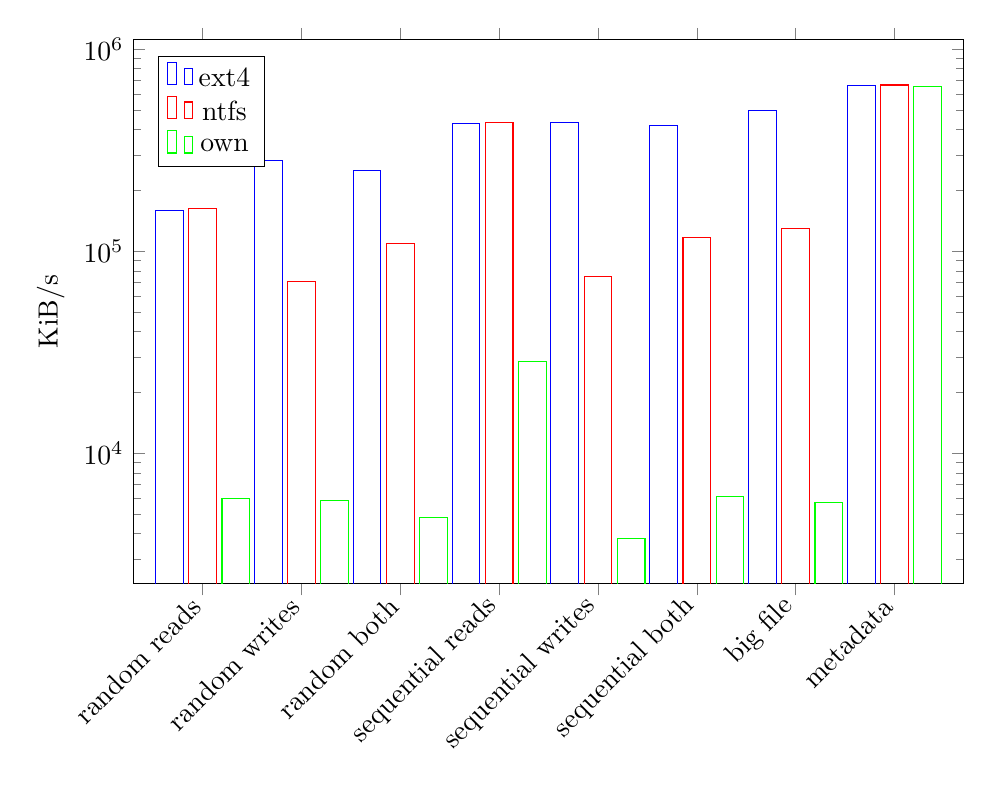
\begin{tikzpicture}
\begin{axis} [
    % TODO: add labels on data (useful)
    ybar, ymode = log,
    ylabel = {KiB/s},
    % nodes near coords,
    % nodes near coords align = {vertical},
    % enlargelimits=0.1,
    width=\textwidth, height = 0.7\textwidth,
    symbolic x coords = {
        random reads, random writes, random both,
        sequential reads, sequential writes, sequential both,
        big file, metadata
    },
    x tick label style = {rotate = 45, anchor = east},
    legend pos = {north west}
]

    % ext
    \addplot[
        draw=blue
    ] coordinates {
        (random reads, 159403) (random writes, 280917) (random both, 250539)
        (sequential reads, 430421) (sequential writes, 432469) (sequential both, 417792)
        (big file, 497323) (metadata, 663893)
    };

    % ntfs
    \addplot[
        draw=red
    ] coordinates {
        (random reads, 162133) (random writes, 70519) (random both, 109670)
        (sequential reads, 431445) (sequential writes, 74684) (sequential both, 116395)
        (big file, 128956) (metadata, 664576)
    };

    % own
    \addplot[
        draw=green
    ] coordinates {
        (random reads, 5963) (random writes, 5812) (random both, 4820)
        (sequential reads, 28331) (sequential writes, 3799) (sequential both, 6104)
        (big file, 5693) (metadata, 651947)
    };

    \legend{ext4, ntfs, own};

\end{axis}
\end{tikzpicture}

            \label{fig_benchmark}
        \end{figure}

        The ext4 and ntfs controls appear to behave as expected. Their
        performance is comparable although ntfs performs worse across the board
        as it is natively implemented on Windows and the Linux driver has
        historically been lagging behind. Regardless, the ext4 results are a
        best case maximum whereas the ntfs ones are a more realistic
        representation of an in-kernel but imperfect filesystem.

        The proposed filesystem's performs an order of magnitude lower across
        the board. As discussed in the design stage (\ref{sec_design})
        performance was expected to be worse. Random reads and writes are of
        comparable speed. This is not surprising, as the code paths they take
        are similar. Each access needs to have its destination resolved and
        then data written in the same way. Interestingly, however, sequential
        reads are about an order of magnitude higher than the overall
        perfomance of the filesystems and the corresponding sequential writes.
        This cannot be attributed to drive assymetry, as the difference tends
        to be linear in SSDs \cite{servethehome_review}. Ext4 handles both
        workloads identially, indicating that is not the case. The ntfs-3g
        driver is a reverse engineering effort of the proprietary ntfs
        filesystem and has been notorious for having a problematic
        implementation. To confirm this, we perform profiling analysys in
        \ref{sec_perf}.

        The large file access is in line with the combined sequential test
        indicating that further increases of file size do not reduce
        performance. Finally, the metadata benchmark is surprising as it is in
        line with ext4 and ntfs. This is tahnks to directory and inode files
        having a count at the start of the file so finding a free slot is a
        very fast operation.

    \section{Profiling analysys}
        \label{sec_perf}

        To investigate why the performance is what it is the filesystem was
        profiled with perf. Perf is powerful Linux tool (part of the kernel)
        for program profiling. It can produce performance statistics for
        hardware (cache hits, idle CPU cycles etc) and for sofware (call
        graphs, call frequency, work in each subroutine etc.) \ref{perf}.

        A single profile was taken with \monospace{perf record -g
        <filesystem>}. For a workload, a full run of the benchmark was used
        \ref{sec_benchmark}. Then resulting 147Mb profile was analysed with
        \monospace{perf report -n --children} and \monospace{perf report -n
        --no-children}.

        Unsurpsiginly, most of the time is spent in the kernel (upwards of
        90\%). However, looking into which subroutine enters the kernel (with
        \monospace{--children}) has interesting results. The biggest time
        consumer is, as expected the file access subroutine
        (\monospace{do\_read\_write\_full()}).  However, in it the block
        read/write subroutines (\monospace{read\_block()} and
        \monospace{write\_block()}) do not make up even a quarter of the time
        spent. Instead, on overwhelming majority of the time is spent in btree
        accesses (\monospace{btree\_lookup64()} in this case). Upon inspecting
        the code this is due to two reasons: First, each block is located
        independently of all others and the sequential nature of the \bplustree
        is not utilised (see \ref{sec_btree} design or impl?). Second, large
        writes are handled like a sequence of small writes (with
        \monospace{do\_read\_write\_block()}). Even if sequences of blocks
        could be utilised they could not be observed by the read/write
        subroutine as it never receives them. As virtually all accesses in this
        filesystem relate to a file (\ref{sec_files}), which are accessed with
        these subroutines, all workloads behave identially porrly.

        Knowing this, to explain the sequential read anomally is not hard. With
        this arrangement reading any file will always be faster as it never
        needs to perform file expansion which requires allocation for a small
        speedup as this is un infrequent occurence. It will also, however,
        bypass the file lookup to find the inode itself to begin the read. In
        effect this removes a level of (inefficient) indirection recovering
        about half of the lost performance due to the poor use of the btrees.
        The sequential writes perform poorly because they make up the lost
        level of indirection by expanding the file in a similar manner,
        degrading performance about the same amount that was gained.

        From this analaysys there arises a corollary: allocation cannot be
        fast. And in fact this is the reason why even the largest test is
        relatively small for today's standards. Since all reads and writes are
        treated as individual requests with the size of a block, allocating a
        gigabyte of space requires about 268 million calls to the allocation
        subroutine. Since it is also slow, the results are untenable.
        % explain the 268 mil figure

        do a complexity analysys

        Benefit: simple impl. The kernel has all of that so it's fast.

% actual percents. TODO: put in listing?
% -   93.79%     0.01%            36  filesystem   filesystem            [.] do_read_write_full
%    - 93.78% do_read_write_full
%       - 93.55% do_read_write_block
%          - 86.10% get_pblock_of_byte
%             + 86.10% btree_lookup64
%          + 6.44% file_add_space
%          + 0.61% __libc_pread

        TODO: full perf availble in???
        say implementation is bad, how its bad but don't suggest anything else. That's a discussion

        IDK where to put this:

        The overall poor performance cannot be attributed to a single factor,
        but it is rather a combination of many things stacking with each other.
        First, the above mentioned sequential performance affects the entirety
        of the filesystem, including random accesses. This is beceause every
        file needs to have its inode located in the i-list. Since this is a
        single contiguous file accessing it is of sequential nature. Then, this
        file is linear. Searches through it are of linear complexity. The
        logarithmic speedup of the B-trees is irrelevant when all blocks need
        to be acccessed, especially when they are trieated as random. The same
        applies for direcoties, as their implementation is identical so
        directory lookups get a double slow down. Further, allocations slow
        things down further as described before. Finally, caching is not
        present so any neighbouring or repeat accesses are treated as
        completety independent and fresh leaving lots of performance on the
        table.

        essentially even random accesses are sequential and we already saw why those are slow

    \section{Design of the filesystem}
    % \subsection{Suitability of design as an FS}
    % maybe in discussion?

    \section{Failure simulation}

        To simulate failures we use a similar approach to the benchmarking.
        Once again, we use fio. This time a 5 minute stress test is perfomerd.
        It has two jobs which run concurrently. The first one preforms the same
        1GB combined read and write load while the second one creates and
        removes 100 files repeatedly. While this test is running a script goes
        over the first drive in the array and flips a random number of bits on
        each block up to a maximum of 100 in an infinite loop.

        As expected, the 5 minute stress test runs without any user visible
        errors. The filesystem detects and corrects all corrupt blocks and
        returns correct data stored on the redundant drives.

        % TODO: add a figure with the debug output that the error was detected and fixed

    \section{Design of the redundancy}
    % \subsection{Suitability of design for error correction}
    % \section{Reliability}

        As shown experimentally, the integrity guarantee works. Theoretically,
        best case security of the 256 bit hashes are $2^128$ bits. Theoretical
        attacks on reduced versions of the function put this at $2^126$
        \cite{sha2_security}, \cite{https://eprint.iacr.org/2016/374.pdf}. At
        this time sha-256 does not have any known collisions. So for the
        purposes of this project we consider it as secure with $2^126$ bits of
        security (we select the lower bound for safety).  Thus the probability
        that a faulty sector results in a hash collision will be at most
        $2^-126$. It is important to note that errors are not entirely
        arbitrary but rather follow some patterns \ref{the place I explain
        this} and are likely to have very few bits changed. Therefore for
        normal wear and tear the probability of a collision is likely to be
        much lower due to the avalanching effect of the funciton \cite{one of
        the above?}, however, this has not been theoretically verified and
        shall not be relied upon.

        In the event of malicious loads like a rowhammer like attack
        \cite{https://www.usenix.org/system/files/conference/woot17/woot17-paper-kurmus.pdf}
        the security is likely to be lower as the attacker can craft the
        payload more carefully. However, the checksumming of the data provide a
        barrier to pulling off such an attack despite the lowered security
        (much like a canary in compilers). We can conclude that even if
        security of the hash under malicios attack is greatly diminished there
        is still a great security benefit.

        Unlike ZFS \ref{sec_ZFS}, this filesystem does not chain checksums.
        Therefore it is possible to change two blocks (one data and one hash)
        in such a way that the checksum is still valid. ZFS's chaining of
        hashes mitigates against this. However, the chance of this happening is
        astronomically low. As the errors are independent on SSDs \ref{that
        again} the likelyhood of that happening with sha256 will be $2^252$.
        This is a valid issue to have with short (eg. CRC) checksums however
        with long hashes this issue can be safely ignored.


\include{./chapters/results}

% Adds references to the table of contents.
\addcontentsline{toc}{chapter}{References}

% All your bibtex entries should go in the file called "refs.bib".
\bibliography{refs}

% All appendices you have go in a file called "appendices.tex".
\begin{appendices}

%
% The first appendix must be "Self-appraisal".
%
\chapter{Self-appraisal}

    % <This appendix should contain everything covered by the 'self-appraisal'
    % criterion in the mark scheme. Although there is no length limit for this
    % section, 2---4 pages will normally be sufficient. The format of this
    % section is not prescribed, but you may like to organise your discussion
    % into the following sections and subsections.>

    \section{Critical self-evaluation}

    \section{Personal reflection and lessons learned}

    \section{Legal, social, ethical and professional issues}

    % <Refer to each of these issues in turn. If one or more is not relevant to
    % your project, you should still explain {\em why} you think it was not
    % relevant.>

        % TODO ask should i keep copyright?
        \subsection{Legal issues}
            \label{app:licence}

            This project has one legal issue. It borrows code from the Linux
            kernel which is licensed undre the GNU General Public License
            version 2 (GPL v2). This license is restrictive to the extent that
            it mandates any modification of borrowed code to be released under
            the terms of the same license. To comply with this requrement, the
            borrowed B-tree code maintains all license and copyright notices.
            Further, the whole project adopts the GPL v2.


        \subsection{Social issues}

            The project does not address nor does it further any social issues.
            As a piece of infrastructure it does not relate or benefit other
            disciplines such as education. It also does not further issues of
            crime, bullying, privacy or (in)equality. The project is open
            source and available to all regardless of skill, social or cultural
            background. It cannot be used to facilitate criminal activity
            insofar as any data storage system can.

        \subsection{Ethical issues}

            This project is not affected by ethical issues. That is becuase it
            does not deal with human subjects directly and where it is
            indirectly involved with humans, it provides no new tools where an
            ethical issue might arise. Particularly, this project does not deal
            with the particularly sensistive field of artificial intelligence
            and its use of cryptography is limited to hashing. Any possible use
            of the project is already covered by exisiting filesystems such as
            EXT4 in regards to efficiency or ZFS for reliability. Where
            features that ZFS provides can be used for criminal and morally
            dubous activity, like data integrity, are meant to be a weaker in
            this project from the project definition (\autoref{sec:problem}). Where
            features that EXT4 provides can be used for similar purposes, like
            large scale deployments, this filesystem purposefully scales back
            on to provide redundancy.

        \subsection{Professional issues}

            This project has been developed in accordance with the principles
            of the British Computer Society's (BSC) code of conduct. In
            particular, it aims to be further the public interest in that it
            provides a useful tool for home use...
            % TODO:


%
% Any other appendices you wish to use should come after "Self-appraisal". You can have as many appendices as you like.
%
\chapter{External Material}

    % <This appendix should provide a brief record of materials used in the
    % solution that are not the student's own work. Such materials might be
    % pieces of codes made available from a research group/company or from the
    % internet, datasets prepared by external users or any preliminary
    % materials/drafts/notes provided by a supervisor. It should be clear what
    % was used as ready-made components and what was developed as part of the
    % project. This appendix should be included even if no external materials
    % were used, in which case a statement to that effect is all that is
    % required.>

    \begin{enumerate}
        \item B-trees from Linux
    \end{enumerate}

\end{appendices}


\end{document}

